% Source: src-b19b233abb266d1b051ded3c332a399c1722d8192d07ce1bf2234dda57bd25bc, PDF p.1.
% Square, disk, and a segment joining the two opposite sides; schematic only.
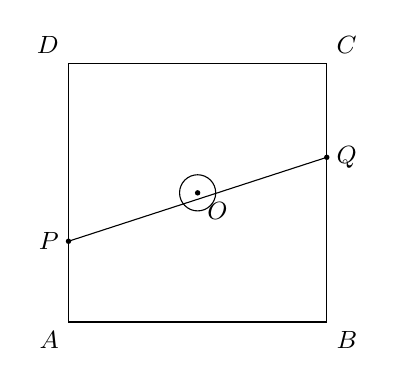
\begin{tikzpicture}[scale=0.82, every node/.style={font=\small}]
  \coordinate (A) at (0,0);
  \coordinate (B) at (4,0);
  \coordinate (C) at (4,4);
  \coordinate (D) at (0,4);
  \coordinate (O) at (2,2);
  \coordinate (P) at (0,1.25);
  \coordinate (Q) at (4,2.55);
  \draw (A)--(B)--(C)--(D)--cycle;
  \draw (O) circle[radius=0.28];
  \draw (P)--(Q);
  \fill (O) circle (1.2pt);
  \fill (P) circle (1.2pt);
  \fill (Q) circle (1.2pt);
  \node[below left] at (A) {$A$};
  \node[below right] at (B) {$B$};
  \node[above right] at (C) {$C$};
  \node[above left] at (D) {$D$};
  \node[below right] at (O) {$O$};
  \node[left] at (P) {$P$};
  \node[right] at (Q) {$Q$};
\end{tikzpicture}
